\documentclass[letter,12pt]{article}
\usepackage[letterpaper,right=1.25in,left=1.25in,top=1in,bottom=1in]{geometry}
\usepackage{setspace}

\usepackage[utf8]{inputenc}   % allows input of special characters from keyboard (input encoding)
\usepackage[T1]{fontenc}      % what fonts to use when printing characters       (output encoding)
\usepackage{amsmath}          % facilitates writing math formulas and improves the typographical quality of their output
\usepackage[hyphens]{url}     % adds line breaks to long urls
\usepackage[pdftex]{graphicx} % enhanced support for graphics
\usepackage{tikz}             % Easier syntax to draw pgf files (invokes pgf automatically)
\usetikzlibrary{arrows}

\usepackage{mathptmx}           % set font type to Times
\usepackage[scaled=.90]{helvet} % set font type to Times (Helvetica for some special characters)
\usepackage{courier}            % set font type to Times (Courier for other special characters)

\usepackage{rotating}         % sideway tables and figures that take a full page
\usepackage{caption}          % allows multipage figures and tables with same caption (\ContinuedFloat)

\usepackage{dcolumn}          % needed for apsrtable and stargazer tables from R to compile
\usepackage{arydshln}         % dashed lines in tables (hdashline, cdashline{3-4}, 
                              %see http://tex.stackexchange.com/questions/20140/can-a-table-include-a-horizontal-dashed-line)
                              % must be loaded AFTER dcolumn, 
                              %see http://tex.stackexchange.com/questions/12672/which-tabular-packages-do-which-tasks-and-which-packages-conflict

\usepackage{amssymb}          % has nicer empty set \varnothing, among much much more

%FOR SPANISH FORMATTING (HYPHENATION ETC.)
%% \usepackage[spanish]{babel}
%% \addto\captionsspanish{\renewcommand{\figurename}{Diagrama}} % cambia Figura por Diagrama

\usepackage[longnamesfirst, sort]{natbib}\bibpunct[]{(}{)}{,}{a}{}{;} % handles biblio and references 
%% \AtBeginDocument{\renewcommand\harvardand{y}} % change 'author and author' by Spanish 'author y author'

\newcommand{\mc}{\multicolumn}

%% TO ADD NOTES IN TEXT, PUT % BEFORE THE ONE YOU WANT DISBALED
%\usepackage[disable]{todonotes}                            % notes not showed
\usepackage[colorinlistoftodos, textsize=small]{todonotes} % show notes
\newcommand{\emm}[1]{\todo[color=red!15, inline]{\textbf{Eric:} #1}}
\newcommand{\am}[1]{\todo[color=green!15, inline]{\textbf{Alejandro:} #1}}

\begin{document}

% \title{The removal of single-term limits, redistricting, and name recognition in Coahuila's state races}
\title{Redistricting and the separation of incumbency and campaign effects: name recognition in Coahuila\thanks{We thank participants of the IV Encuentro del Grupo de Estudios Legislativos de ALACIP in Mexico City for comments and critiques. We are grateful for the generous support of the Asociación Mexicana de Cultura A.C. The authors bear full responibility for errors and limitations in the study.}}
\author{Eric Magar  \\ ITAM \and
        Alejandro Moreno \\ ITAM 
}
\date{\today}
\maketitle

%\begin{center} \textbf{$\rightarrow$~~Preliminary draft~~$\leftarrow$} \\ (please inquire for new version, \small{\url{emagar@itam.mx}})  \end{center}

\begin{abstract}
\noindent Estudiamos el reconocimiento del nombre de candidatos al Congreso del estado de Coahuila en 2017. El fenómeno ha sido asociado con el esfuerzo del representante en su distrito para preservar su reelegibilidad. Aprovechamos la redistritación del estado que antecedió a la elección para detectar diferencias en reconocimiento atribuibles al efecto del ocupante y no al efecto de campaña. Aunque la cobertura muestral de la encuesta preeelectoral que usamos impide una separación cabal de los dos efectos, detectamos diferenciales en reconocimiento de nombre significativos y consistentes con la teoría. Ofrecemos tres diseños de investigación alternativos para que futuros estudios de opinión separen el efecto de ocupante (\emph{incumbency effect}) en elecciones que permitirán la reelección consecutiva a partir de 2018 en México. 
\end{abstract}


\onehalfspacing

\section{Introduction}

\noindent Mexico inaugurates the consecutive reelection of lawmakers at the state and federal levels, and of municipal governments in all but two states.  For eight decades, every elected officer had to vacate the seat at the end of the term. Reelection is a major change in electoral institutions. Political scientists in American politics see it as the cornerstone of democratic accountability, the key of what \citet{madison.1788} called external checks to the government.\footnote{See \citet{schlesinger.1966}, \citet{mayhew.1974}, \citet{fenno.1978}, \citet{cain.etal.1987}, \citet{mccubbins.sullivan.1987}, \citet{cox.mccubbins.1993}, \citet{weingast.marshall.1988}, \citet{jacobson.1997}, among others.} Those with ambition to keep their job can stay another term if they convince constituents to support them again. The representative delivers in exchange for votes. 

From the U.S./ standpoint, institutional change adopted along the 2014 electoral reform has potential to instill much welcome oxigen to representation relations of Mexico's young democracy. But a comparative perspective serves as a reminder that there is no guarantee that such potential will be fulfilled. While most Latin American democracies allow legislative reelection, few exhibit return rates even remotely comparable to those observed in the U.S. Congress. In fact, pesimistic forecasts of the irrelevance and likely failure of Mexico's reform accompanied its adoption \citep{merinoFierroZarkin2013Blog}. 

The paper elaborates reasons to be optimistic and those to be pessimistic, and examines the case of Coahuila, a northern state bordering the U.S.\footnote{There is institutional variance among states. See \citet{magarInstReel.2017}.}

\section{Political ambition and democracy}

\noindent Contemporary legislative studies generate key hypotheses from Mayhew's \citeyearpar{mayhew.1974} model of lawmaker. The iconic work on the electoral connection of members of the U.S.\ Congress presents legislators as automatons with a unique goal: reelection. The crucial premise in the argument is motivational: only one spring moves the incumbent, the ambition to stay another term in office. Mayhew does not deny that other worries might leave incumbents sleepless---turning some prioritary program into policy, climbing the chamber's hierarchy, her historical legacy are just some examples. But none could be achieeved if the incumbent failed at her attempt to reelect. Despite its parsimony, the model explains most activity that representatives engage in while in Congress. 

Another premise is instrumental: reelection is a function of the incumbent's reputation among constituents. In personalistic systems, such as the U.S., reputation is mostly individual---to such degree that Mayhew discards the possibility that heterogneous American paties could be of theoretical interest \citep[but revisionists rescued party relevance in Myhew's framework,][]{cox.mccubbins.1993,aldrich.1995}. The instrumental premise merits three comments. 

First, it does not involve every constituent in the district but a subset. Groups making reelection much harder if they dropped their support for the incumbent are more important than others. \citet{cox.mccubbins.1986} call them \emph{core constituents}. From this perspective, it is rational and easier to work in preserving a coalition that made you win than attempting to build a new one.

Second, coalition maintenance requires delivering results, channeling new benefits to the core while preserving existing ones. As in all humen relations, perceptions matter as much as substance: the core must give the incumbent credit for delivering. 

With collective production goods, where each member's effort is not immeadiately evident, the allocation of responsibility is far from automatic. Success has many parents. Thus the importance of particularistic goods, in contrast to more universalitic ones. Their distinguishing trait is that their production and/or delivery depends on the incumbnt's personal effort \citep{haggard.mccubbins.2001}. Classic examples are from \citet{cain.etal.1987}: constituency service (service responsiveness) and spending earmarked for the district (allocation responsiveness). Incumbents have full control to direct pork where the political logic indicates, creating (this is crucial) a responsibility link.

To the extent that Mayhew's logic intersects with ascription problems, theory expects legislators to devote substantial time to cultivate their personal vote through delivery of particularistic goods. As a result, a closer link develops between lawmaker and her core constituents than the rest od the citizenry. As a consequence, better incumbent's name recognition is expected in the district than beyond. 

%La noción de ambición política de Mayhew es apropiada para el sistema mayoritario norteamericano, con su característico acceso competitivo y descentralizado a la boleta y carrerismo legislativo. Pero no es necesariamente apropiada para otros sistemas. Pero estos no son rasgos universales. 

%\citet{schlesinger.1966} revisó el modelo para distinguir dos clases de ambición relevantes para el estudio, la estática y la progresiva. En Mayhew hay sólo estática (permanecer en el Congreso), pero también hay políticos que aspiran a elegirse en puestos distintos. Hay evidencia de que el esfuerzo por cultivar votantes coincide con la ambición del ocupante \citep{micozzi.accountability.2013,samuels.2003}. 

%Usaremos estos elementos teóricos para guiar nuestro estudio de los candidatos a diputado local de Coahuila.

\section{A Minimal Effects Hypothesis}

\begin{center}
\begin{singlespacing}
  We face the possibility of approving reelection \\
  while failing to meet its goal, that is true \\
  representation and evaluation by voters \\
  --Senator Ríos Piter\footnote{``Estamos en la posibilidad de que se apruebe la reelección y de que no se cumpla el objetivo, que es la verdadera representación y evaluación por parte de los votantes'', see \url{http://www.diputados.gob.mx/sedia/biblio/prog_leg/135_DOF_10feb14.pdf}.}
\end{singlespacing}
\end{center}

\noindent It is far from evident that the North American electoral connection model can be extended to the Mexican democracy. Sceptics feed on two lines of argument, the partisan padlock and a more general lack of interest for reelection. We elaborate them. 

\subsection{The partisan padlock}

\noindent Reformers in 2014 gave the right of reelection not to the representative but the party. Mexican incumbents can face constituents again in a general election if, and only if, the party that elected them to office nominates them again. This ``padlock'', as it has been called, give the party nomenklatura an absolute veto on the representative's renomination, \emph{even by other parties}.\footnote{Until the Supreme Court declared it unconstitutional, Brazil's \emph{candidato nato} clause imposed the reverse relationship between party and representative, giving the second power to override the leadership veto on renomination \citep{mainwaring.1991}. The United Kingdom uses a mix, giving the national and district parties mutual vetoes on nomination [*cite].}

As a consequence, the mayor or legislator sensing tension between constituents' and party leaders' interests will face a predicament. Siding systematically with constituents will expose her to the wrath of the party and, as retaliation, she may be prevented from being on the ballot---the same source of discipline towards legislative leaders as single term limits \citep{weldon.1997}. \citet{merinoFierroZarkin2013Blog} go as far as claiming that the padlock will fully remove the beneficial effects of consecutive reelection. 

The institution looks intended to lessen incumbents' independence. As often happens with negotiation between legislative parties, reformers' intentions are easier to gauge by listening to opponents --- the introduced bill's summary (\emph{exposición de motivos}) does not even mention the padlock. Their plenary interventions seem to confirm leaders' fears of losing the firm grip they have held upon elected officeholders.\footnote{The diario de los debates for the December 3rd, 2013 session, when the reported bill was discussed and approved, registers the intervention (for the report) of Sen.\ Javier Corral (PAN--Chihuahua). He addresed legislators' opportunism against their parties: ``I would have preferred a direct reelection'' he claimed, ``but I also believe that the report mitigates a phenomenon that cannot be ignored, that of political turncoats'' (``Me hubiera gustado una reelección directa, pero también creo que el dictamen se encarga de un fenómeno que no podemos negar, el transfuguismo político''). Later on, Sen.\ Armando Ríos Piter (PRD--Guerrero) further elaborated while introducing a failed amendment to delete the padlock: ``it is important to drop it'', he argued, ``[b]ecause if we wish the evaluation be made by citizens we cannot let it depend on a political party'' whom, in roll calls, will be watchful that the ``legislator does not escape the sheepfold'' (``es importante quitar[lo]... [p]orque si queremos que la evaluación la hagan los ciudadanos pues no podemos dejar que dependa de un partido político'' que, en las votaciones, velará por que el ``legislador no se salga del redil.'' See \url{http://www.diputados.gob.mx/sedia/biblio/prog_leg/135_DOF_10feb14.pdf}.}

%Siguiendo a los apologistas de la reelección consecutiva en México desde \citet{lujambio.1996} (quizás antes), subraya un esperado efecto benéfico en la profesionalización de los legisladores.\footnote{\citet{dworak.legisladorAexamen.2003,campos.1996,careaga.1996}; \url{http://www.animalpolitico.com/blogueros-vision-legislativa/2013/12/04/reeleccion-legislativa-historia-y-estadisticas/}.} Menciona someramente el argumento de la conexión electoral, pero mantiene silencio sobre las razones del candado partidista. 

%Dip. Ricardo Monreal (oponiéndose tanto al candado como a la reelección): Si se mantiene la redacción tal y como está, lo único que se va a promover es fortalecer el cacicazgo político, fortalecer la partidocracia y generar una casta que va a ser difícil sacudirse de ella. 

Discussion so far has been black or white: whether or not consecutive reelection will develop a U.S.-style electoral connection in Mexico. A shade of grays seems more more attractive theoretically. Fully canceling the electoral connection requires incumbents /emph{fully} lacking resources to defend from the leadership. Some politicians are, no doubt, in such a position --- freshmen, personal appointees, etc. But \emph{any} resource of this nature opens room for negotiation between incumbent and party. This is the essence of legislative party theory \citep{cox.mccubbins.1993,aldrich.rohdeCPG2001}.

One resource we have in mind is electoral competitiveness. \citet{zallerprizeFighters} models incumbents as prize fighters and the electoral arena as a selection mechanism: winners demonstrate better adaptation than defeated challengers. Personal electoral machines, political dynasties, or personal charisma are some elements feeding incumbents ``natural advantages''. 

From this perspective, a party can stubbornly prevent a prize fighter's attempts to be on the ballot towards reelection, but does so the peril of losing the district. Given the padlock, the incumbent will be prevented from running at all in the consecutive race, but has the option of moving the machinery and resources to another party.\footnote{A sketch of a model is as follows. The vote share in the district or municipality has three components: $P + C + O = 100$ where $P$ is the party's expected vote without the incumbent's machine, $C$ is the vote share that the incumbent can mobilize personally, and $O$ is the opposition's expected vote share. Any candidate controlling $C \ge |P-O|$ votes is in a position to impose his re-nomination to party leaders. Alternation in many states, districts, and municipalities since 1989 has been the result of such defections and splits towards another party [Ver manuscrito q me dio FEE].}

Those with enough resources should therefore negotiate with the party without removing the electoral connection completely. In any event, whether or not the shades of gray argunment is correct can be resolved empirically. This paper does a first attempt to test it. 

\subsection{Lack of interest towards reelection}

\noindent Pessimists also feed on reelection apathy. The lack of interest for reelecting to the assembly is so frequent among Latin American politicians that \citet{morgenstern.2002b} and \citet{micozziPhD2009} argue in favor of distinguishing between static and progressive ambitions. A look towards reelection rates in some of the continent's cases shows the usefulness of Schlesinger's \citeyearpar{schlesinger.1966} original notion.

%% \begin{table}
%%   \centering
%% %  \begin{tabular}{lccc}
%% %  \begin{tabular}{p{.25\textwidth} p{.18\textwidth} p{.18\textwidth} p{.18\textwidth}}
%%   \begin{tabular}{lccc}
%% %           & \mc{3}{c}{Incumbents and reelection} \\ [-.5ex]
%% %           & seek & succeed & return \\ \hline
%%                          & \mc{3}{c}{Ocupantes (\%) que} \\ 
%%                          & buscaron la & consiguieron    &            \\ [-.5ex]
%%                          & reelección  & reelegirse      & retornaron \\ [-.5ex]
%%     Caso                 & ($a$)       & ($b$)           & ($c=a\times b/100$) \\ \hline \\ [-1.25ex] 
%%     Argentina 1983--2001 & 25          &  76             &     19     \\
%%     Brasil 1995          & 70          &  62             &     43     \\
%%     Chile 1993--2000     & 71          &  83             &     59     \\
%%     EE.UU. 1990--2010    & 91          &  94             &     85     \\ \\ [-1.25ex] \hline
%% %    \mc{4}{p{.79\textwidth}}{\footnotesize{Fuentes: \citet[][:658]{jones.etal.amateurLegis.2002} para Argentina; \citet[][:415--6]{morgenstern.2002b} para Brasil y Chile; \url{https://www.opensecrets.org/overview/reelect.php} para EE.UU.}} \\ \hline
%%   \end{tabular}
%%   \caption{Querer y poder retornar al Congreso de cuatro democracias. La columna (a) reporta el porcentaje de ocupantes de la cámara baja que fueron renominados, la (b) el porcentaje de éstos que se reeligió y la (c) la tasa de retorno. Fuentes: \citet[][:658]{jones.etal.amateurLegis.2002} para Argentina; \citet[][:415--6]{morgenstern.2002b} para Brasil; \citet{naviaIncumbency.2000} para Chile; \url{https://www.opensecrets.org/overview/reelect.php} para EE.UU.}\label{T:retRate}
%% \end{table}

\begin{table}
  \centering
%  \begin{tabular}{lccc}
%  \begin{tabular}{p{.25\textwidth} p{.18\textwidth} p{.18\textwidth} p{.18\textwidth}}
  \begin{tabular}{lccc}
%           & \mc{3}{c}{Incumbents and reelection} \\ [-.5ex]
%           & seek & succeed & return \\ \hline
                             & \mc{3}{c}{Incumbents (\%) who} \\ 
                             & sought      &             &            \\ [-.5ex]
                             & reelection  & reelected   & returned   \\ [-.5ex]
    Case                     & ($a$)       & ($b$)       & ($c=a\times b/100$) \\ \hline \\ [-1.25ex] 
    Argentina 1983--2001     & 25          &  76         &     19     \\
    Brazil 1995              & 70          &  62         &     43     \\
    Chile 1993--2000         & 71          &  83         &     59     \\
    United States 1990--2010 & 91          &  94         &     85     \\ \\ [-1.25ex] \hline
%    \mc{4}{p{.79\textwidth}}{\footnotesize{Fuentes: \citet[][:658]{jones.etal.amateurLegis.2002} para Argentina; \citet[][:415--6]{morgenstern.2002b} para Brasil y Chile; \url{https://www.opensecrets.org/overview/reelect.php} para EE.UU.}} \\ \hline
  \end{tabular}
  \caption{The willing and the able to return to Congress in four democracies. Columns (a) reports the percentage of incumbents in the lower chamber that were re-nominated, column (b) the percentage of them that reelected for another consecutive term, and column (c) the return rate. Sources: \citet[][:658]{jones.etal.amateurLegis.2002} for Argentina; \citet[][:415--6]{morgenstern.2002b} for Brazil; \citet{naviaIncumbency.2000} for Chile; \protect\url{https://www.opensecrets.org/overview/reelect.php} for the U.S.}\label{T:retRate}
\end{table}

Consider, in Table \ref{T:retRate}, the values of three indicators for the Argentine, Brazilian, Chilean, and U.S.\ Congresses. The first indicator is the percentage of incumbents who ran again for the same office at the end of their terms (column a), capturing  static ambition: incumbents who bet for pursuing a career in the chamber and therefore tried to repeat in office. Variation is noteable. If 9 out of 10 U.S.\ incumbents regularly manifest static ambition, a bare quarter did in Argentina since the return to democracy. Brazil and Chile ocupy intermediate positions, although more similar to the U.S.\ than Argentina. 

Because desire is not the same as ability, the Table also reports the conditional success rate (that is, among renominated incumbents only, column b). The case of the U.S.\ strikes the eye again, where 94 percent fulfilled their ambition. Below, Chilean incumbents' conditional success rate, at 78 percent, is quite impressive too. In Brazil is was more moderate, at 62 percent. The product of indicators (a) and (b) returns the third one: incumbents'rate of consecutive return to the chamber (column c). The four case cover most of the range: from 19 percent in Argentina (despite a pretty high conditional success rate) to 85 percent in the U.S.

Incumbents without static ambition fall in two categories: those with progressive ambition (who ran for a different office) and those with no ambition (who retired). The question of interest is which category will Mexican incumbents mostly populate and which they will shun in the near future? Will there be little if any static ambition, as in Argentina? It is improbable that is becomes near universal, an in the United States, but is there room to become similar to Brazil or even Chile?

\begin{table}
  \centering
  \begin{tabular}{lc}
    Year &  \% returned  \\ \hline \\ [-1.25ex]
    1916 (Constitutional Assembly) &          --- \\
    1917 &           18 \\
    1918 &           25 \\
    1920 &           15 \\
    1922 &           26 \\
    1924 &           25 \\
    1926 &           30 \\
    1928 &           40 \\
    1930 &           42 \\
    1932 &           27 \\
    1934 (single-term limits effective) &            0 \\ [-1.25ex] \\ \hline
  \end{tabular}
  \caption{Reelection in the Chamber of deputies up to 1934. Source: \citet{godoy.reeleccion.2014}.}\label{T:1920s}
\end{table}

History suggests that there might be. Table \ref{T:1920s} reports the return rate of federal deputies observed by \citet{godoy.reeleccion.2014} in the years prior to the adoption of single-term limits. The evidence is interesting and suggestive. The start of the series, when the Revolutionary constitution was adopted, bears similarity to present-day Argentina (just 18 percent of constitutional assembly members became deputies in the XXVIIth Legislature of 1917--18). But the return rate grew at an accelerated pace in the second hald of the 1920s. By 1928 it had doubled, reaching 40 percent. It then stabilized and dropped sharply when the reelection ban could be foreseen.\footnote{46 percent of the congressional districts were eliminated before the 1930 election---from 281 members, the chamber dropped to 153 only, see \citet[][:23]{godoy.reeleccion.2014}. Since the return rate remained at 42 percent despite the sharp drop in the denominator shows that a good number of incumbents with static ambition were targeted and left orphans with no district.} 

%Es indudable que la cláusula podría anular la independencia del legislador para defender los intereses de sus representados. Pero no hay tampoco garantía de ello. , Y la posibilidad de que no haya interés. En ambos casos, la pregunta es empírica. Campeones y Godoy.

%Este trabajo lleva a cabo un estudio preliminar. Aprovecha elección Coahuila 2107, primera y única hasta ahora con ocupantes en la boleta. Estudiamos una encuesta y reconocimiento de nombre. Si el diseño de la presente investigación tiene una limitación fundamental, el trabajo ofrece la ventaja de describit con detalle el diseño que permitirá superar la limitación. Bienvenido para estudiar los 24 estados que podrán tener ocupantes en la boleta en 2018. 

\section{Redistricting as source of hypotheses}

\noindent We examine name recognition in Coahuila, whose incumbents legislators could reelect consecutively in 2017. As in the rest of the country, the Instituto Nacional Electoral (INE) redrew the boundaries of the sixteen state legislative districts in 2015 \citep{trelles.etalDatosabiertos.pyg.2016}. We exploit this coincidence to generate falsifiable hypotheses. The idea is simple. Incumbents who sought to return to office competed in districts more or less different from those they had represented. We hope that the degree of disimilarity in their constituents manifests in differenciated patterns of name recognition. 

\begin{figure}
  \centering
    \usetikzlibrary{calc}
    \begin{tikzpicture}
      \draw (0,0)  ellipse (3 and 2);
      \node[sloped,above] at ($(0,0)+(90:3 and 2)$) {\textsc{father}};
      \draw (3,0) ellipse (3 and 2);
      \node[sloped,above] at ($(3,0)+(90:3 and 2)$) {\textsc{son}};
      \draw (-3.5,-3) rectangle (6.5,3);
      \node [text width=2cm, text centered] at (-1.25,0)   {$l=$ land lost};
      \node [text width=2cm, text centered] at (4.25,0)    {$i=$ land incorporated};
      \node [text width=2cm, text centered] at (1.5,0)  {$r=$ land retained};
      \node at (1.5,-2.5) {$n=$ no man's land};
    \end{tikzpicture}
    \caption{Four clear and distinct lands arise from redistricting. \textsc{Father} and \textsc{son} represent 2014 and 2017 map districts, respectively.}\label{F:venn}
\end{figure}

To set the test, we start by identifyng `father' and `son' districts. We construe district genealogy as \citet{cox.katz.2002} do. We compare, one-by-one, districts in the new maps (the offspring) to those in the old map, in order to detect which they share the most voters with. This is the district's father. Figure \ref{F:venn} pictures a Venn diagram of a father  (from the 2014 map) and son (from the 2017 map). Ovals are simplified versions of district boundaries (minus geographic accidents typical of real-world maps). Four terrains can be distringuished. Intersection $r$ is land (and the voter who live there) from the father that the son has retained. By construction, $r$ is never empty (else the district would have no father). To its left is land $l$ from the father that the son has lost by the redistricting, and to its right lies land $i$ that the son has incorporated from one or more other old-map districts. Lands $l$ and $i$ represent change in the map, and one, the other, or both could be empty. Land $n$ not belonging to any of the ovals is no man's land, with no interest whatsoever for the incumbent at hand. 

The approach quantifies the degree of change in an incumbent's electorate brought by redistricting. Comparing the land father and son share in common with land lost and gained yields an index of district similarity $S_j$ for district $j$. If $\texttt{father}_j$ and $\texttt{son}_j$ denote, respectively, voters in the father and son districts, then $S_j = \frac{\texttt{father}_j \cap \texttt{son}_j}{\texttt{father}_j \cup \texttt{son}_j} = \frac{r}{l+r+i}$. The index reaches a maximum value $S_j=1$ when father and son are identical (i.e., $l=i=\varnothing$) and drops gradually as intersection $r$ shrinks relative to $l+i$. The index tends to zero when father and son intersect minimally (zero is never reached because $r$ is never empty).

\begin{table}
  \centering
\begin{tabular}{llrcc}
 Son district                &  Father district            &       &                        & Revealed          \\ [-.5ex]
 (2017)                      &  (2014)                     &  $S$  & Incumbent              & ambition          \\ \hline
\\ [-1.2ex]
 \textsc{xii}-Ramos Arizpe   & \textsc{v}-Ramos Arizpe     & 1.000 & Lily Gutiérrez B.      & \textbf{static}   \\
 \textsc{i}-Acuña            & \textsc{xv}-Acuña           &  .798 & Georgina Cano T.       & \textbf{static}   \\ 
 \textsc{ii}-Piedras Negras  & \textsc{xvi}-Piedras Negras &  .791 & Sonia Villarreal P.    & progressive       \\ 
 \textsc{x}-Matamoros        & \textsc{vii}-Torreón        &  .705 & Shamir Fernández H.    & none              \\ 
 \textsc{xiv}-Saltillo       & \textsc{i}-Saltillo         &  .700 & Javier Díaz G.         & \textbf{static}   \\ 
 \textsc{ix}-Torreón         & \textsc{viii}-Torreón       &  .650 & Irma Castaño O.        & none              \\ 
 \textsc{vii}-Matamoros      & \textsc{vi}-Torreón         &  .618 & Verónica Martínez G.   & none              \\ 
 \textsc{xvi}-Saltillo       & \textsc{ii}-Saltillo        &  .553 & Francisco Tobías H.    & none              \\ 
 \textsc{iii}-Sabinas        & \textsc{xiii}-Múzquiz       &  .551 & Antonio Nerio M.       & none              \\ 
 \textsc{xiii}-Saltillo      & \textsc{iv}-Saltillo        &  .459 & Martha Garay C.        & none              \\ 
 \textsc{iv}-San Pedro       & \textsc{x}-San Pedro        &  .444 & Ana Isabel D.          & progressive       \\ 
 \textsc{v}-Monclova         & \textsc{xii}-Monclova       &  .408 & Melchor Sánchez F.     & none              \\ 
 \textsc{vi}-Frontera        & \textsc{xi}-Frontera        &  .377 & F. `Lencho' Siller     & progressive       \\ 
 \textsc{xiii}-Saltillo      & \textsc{iii}-Saltillo       &  .236 & José María Fraustro S. & none              \\ 
 \textsc{ix}-Torreón         & \textsc{ix}-Torreón         &  .204 & Luis Gurza J.          & none              \\ 
 \textsc{iii}-Sabinas        & \textsc{xiv}-Sabinas        &  .197 & Martha Morales I.      & none              \\ 
 \\ [-1.2ex] \hline
\end{tabular}
\caption{District similarity index in Coahuila}\label{T:dsi}
\end{table}

We report Coahuila's district simularity in 2017 in Table \ref{T:dsi}. We operationalize $S$ with electoral \emph{secciones} instead of voters. The survey we rely on identified the \emph{sección} where interviewees regitered for voting, so this suffices for th test.\footnote{With our operationalization, $S$'s value is the share of secciones that father and son share vis-à-vis secciones both districts share. If electoral secciones all had identical populations, our operationalization would be identical to Cox y Katz's, who rely on shared population instead of shared secciones. As population heterogeneity rises, so do discrepacncies between both versions of $S$ across districts. Electoral secciones have relatively homogeneous populations: 99 percent had between 100 and 5,700 inhabitants in the 2010 census.} The median district, located between numbers \textsc{iii} and \textsc{xvi}) in the Table, shares 55 percent secciones from the reunion with its father. Similarity looks scant: if the incumbent ran again for consecutive reelection and knew personally every citizen she represented during the term that is expiring, she would recognize only a bit more than half of her new constituents. $S$'s inter-quartile range is .4--.7.

From the electoral connection's perspective, changes of this sort in electoral geography should discourage static ambition among incumbents, pushing them for retirement. And so it happened. We have no evidence to claim that redistricting pushed thirteen of sixteen single-member district incumbents to not seek reelection. But it is a fact that the three who did represented districts with higher similarity indexes (the right-most column in the table reports incumbents' revealed ambition), which is consistent with the electoral connection. Lily Gutiérrez's constituents in Ramos Arizpe in fact changed nothing at all (she ran in the only district with $S=1$). Georgina Cano from Acuña and Javier Díaz from Saltillo retained 8 and 7 of every 10 voters, respectively.  

\begin{table}
  \centering
  \begin{tabular}{cccc}
    & Incumbency & Campaign & Total   \\ [-.5ex]
    & effect     & effect   & effect  \\ \hline
    \\ [-1.2ex]
    1 & $r>i$    & $r=i$    & $r>i$   \\
    2 & $r>l$    & $r>l$    & $r>l$   \\
    3 & $r>n$    & $r>n$    & $r>n$   \\
    4 & $l~?~i$  & $l<i$    & $l~?~i$ \\
    5 & $l>n$    & $l=n$    & $l>n$   \\
    6 & $i>n$    & $i>n$    & $i>n$   \\ \\ [-1.2ex] \hline 
    %% & Efecto &       Efecto &        Efecto \\ [-.5ex]
    %% & del ocupante & de la campaña & total\\ \hline
    %% \\ [-1.2ex]
    %% 1 & $c>a$   & $c=a$  & $c>a$   \\
    %% 2 & $c>p$   & $c>p$  & $c>p$   \\
    %% 3 & $c>y$   & $c>y$  & $c>y$   \\
    %% 4 & $p~?~a$ & $p<a$  & $p~?~a$ \\
    %% 5 & $p>y$   & $p=y$  & $p>y$   \\
    %% 6 & $a>y$   & $a>y$  & $a>y$   \\ \\ [-1.2ex] \hline 
  \end{tabular}
  \caption{Incumbency and campaign effects in name recognition (hypotheses). Cells give expected relations in name recognition in the areas defined in Table \ref{F:venn}. Thus, the first line indicates that incumbency causes higher name recognition among voters in land retained than those in land incorporated, a difference not caused by the campaign effect; combining them gives the reported total effect.}\label{T:hyps}
\end{table}

For our purpose, reistricing opens up room to separate and measure different effects in incumbents' name recognition among constituents, summarized in Table \ref{T:hyps}. Two forces must be distinguished as they operate jointly on name recognition: incumbency (discussed above) and campaign effects.

The bulk of effort in a legislative campaign takes place in the district \citep{langston.nd}. Billboards and wall paintings, printed flier distribution and robocalls, meetings with neighbors alone or in the company of candidates higher in the ticket, or even vote-buying with construction material and debit cards are some examples of focalized effort. The effect in the candidate's name recognition occurs \emph{throughout the district} (i.e., the son). In contrast, the effect of incumbency in name recognition occurs in the area that father and son share. This generates our first predictions.

The probability that a voter picked at random among constituents (in lands $r$ or $i$) recognizes the candidate's name is substantially higher than a voter picked at random from outside the district (in $l$ or in $n$). By itself, the campaign effect generates no difference in recognition between areas $r$ and $i$. Neither does it among $l$ and $n$. The seconf column in Table \ref{T:hyps} reports these predictions. They can be summarized as $r=i>l=n$. 

On the other hand, incumbency has an effect in area $l$ to some degree only. The incumbent used to represent voters in both $r$ and $l$. Upon seeing the new map, she realized having lost fragment $l$ and its voters. She must have adjusted her finite effort: stop cultivating voters in area $l$ in order to start doing it in area $i$. Despite re-balancing, previous effort in $l$ (which includes the effect of the previous campaign) does not immediately vanish. Unlike $r$, whose voters experienced such efort for three full years, area $i$'s experienced it less long. The first column reports these predictions: $r>i$ and $r>l$. 

l ? g

> n

Incumbents running for reelection generate the sum of effects (reported in the third column), challengers generate campaign effects only. Vea el texto.

%% \begin{table}
%%   \centering
%%   \begin{tabular}{lrrrr}
%%                & \mc{2}{c}{Contendió de nuevo}           &           &       \\ [-.5ex]
%%     Diputado   &        en un distrito & en un municipio & Se retiró & Total \\ \hline
%%     de mayoría &                     3 &            3    &        10 &    16 \\
%%     de RP      &                     0 &            3    &         6 &     9 \\ \hline
%%   \end{tabular}
%%   \caption{Ocupantes con ambición estática, progresiva o nula} \label{T:ambition}
%% \end{table}

%El Cuadro \ref{T:ambition} resume la ambición revelada por los legisladores en funciones en Coahuila en 2017. De los dieciséis diputados que representaban un distrito (todos del PRI, que ganó un carro completo en 2014), tres aspiraron a reelegirse como diputados, tres a elegirse como alcaldes, y diez se retiraron. Y tres de nueve diputados de lista aspiraron a volverse alcaldes. A pesar de la posibilidad que abrió la reforma, entre los diputados que no se retiraron, los de ambición progresiva duplicaron a los de ambición estática mostraron ambición progresiva---transitaron la ruta tradicional del llamado ``chapulineo'', que antes era la única disponible.

%Terminología: ocupante es un candidato que ha representado un territorio en el periodo que concluye tras la elección y que compite por la reelección; rival es todo candidato que no es ocupante.  



%\singlespacing

%% \begin{description}
%%   \item [Hipótesis 1] Manteniendo lo demás constante, el reconocimiento de un ocupante sigue los patrones siguientes:
%%     \begin{enumerate}
%%       \item es mayor entre votantes del terreno $c$ que entre los del $h$
%%       \item es mayor entre votantes del terreno $c$ que entre los del $p$
%%       \item es mayor entre votantes del terreno $c$ que entre los del $a$
%%       \item es mayor entre votantes del terreno $p$ que entre los del $h$
%%       \item es mayor entre votantes del terreno $a$ que entre los del $h$
%%       \item es mayor entre votantes del terreno $p$ que entre los del $a$
%%     \end{enumerate}
%% \end{description}

%% \onehalfspacing

%% \singlespacing

%% \begin{description}
%%   \item [Hipótesis 2] Manteniendo lo demás constante, el reconocimiento de un rival sigue los patrones siguientes:
%%     \begin{enumerate}
%%       \item es menor entre votantes del terreno $h$ que entre los demás
%%       \item no muestra diferencias significativas entre votantes de los terrenos $p$, $c$ y $a$. 
%%     \end{enumerate}
%% \end{description}

%% \onehalfspacing


\section{Data and methods}

We analyze a face-to-face survey from May 19--21, 2017 in Coahuila, two weeks before the state legislative election (concurrent with a gubernatorial and municipal races).\footnote{The survey was commissioned to Alejandro Moreno by \emph{El Financiero} newspaper (published May 25). A sample of 1,008 registered voters was interviewed in households. Urban/rural electoral secciones were stratified, then a random sample taken to select 72 points throughout the state where interviews took place. The 95-percent confidence interval of inferences has a $\pm3.1\%$ error. The non-response rate was 32\%.} The survey includes questions on name recognition inspired from \citet{cain.etal.1987}. We coded name recognition indicators for six incumbents in Table \ref{T:dsi} (all representing single-member districts). Three ran for reelection (static ambition) and three for election to municipal office (progressive ambition). We also coded indicators for three proportional-representation lawmakers who ran for municipal office. 

%Encuesta en Coahuila realizada cara a cara en vivienda del 19 al 21 de mayo a 1,008 adultos con credencial para votar vigente. Las entrevistas se llevaron a cabo en 72 puntos de la entidad seleccionados probabilísticamente a partir del listado de secciones electorales del INE previamente estratificadas por criterio urbano-rural. Con un nivel de confianza de 95%, el margen de error de la encuesta es de +/- 3.1%. La tasa de rechazo a las entrevistas fue de 32%. “Los resultados reflejan las preferencias electorales y las opiniones de los encuestados al momento de realizar el estudio y son válidos para esa población y fechas específicas”. Se entrega copia del estudio y sus características metodológicas al Instituto Electoral de Coahuila.

In all cases, we relied on close-ended questions mentioning the incumbent's name while asking interviewees how much they remebered it (see the appendix) to code nine dependent variables. An incumbent's name recognition indicator $\texttt{recognize}_i$ takes value 1 if respondent $i$ expressed remembering his/her name in any degree; 0 otherwise. *Descriptive here.

We analyze name recognition with equation
\begin{equation}
  \begin{split}
\text{logit}(\texttt{recognize}_i) & =    \beta_0
                                       + \beta_1\texttt{retained}_i
                                       + \beta_2\texttt{lost}_i
                                       + \beta_3\texttt{delivered}_i \\
                                     & + \beta_4\texttt{interested}_i
                                       + \beta_5\texttt{smartphone}_i 
                                       + \beta_6\texttt{panista}_i \\
                                     & + \beta_7\texttt{priista}_i
                                       + \beta_8\texttt{morenista}_i
                                       + \text{error}_i.
  \end{split}
\end{equation}
The model includes two geographic indicators: $\texttt{retained}_i$ equals 1 if respondent $i$ is a voter registered in area $r$, 0 otherwise; and $\texttt{lost}_i$ equals 1 if respondent $i$ is a registered voter in area $l$, 0 otherwise. The geographic regressors are mutually-exclusive but not exhaustive, thus avoiding the dummy trap. The omitted category is for respondents in area $n$, so these indicators' coefficients are interpreted against it. The model also includes indicators for incumbent responsiveness ($\texttt{delivered}_i$ equals 1 if the respondent said the incumbent did something for the district, 0 otherwise), for interest in politics ($\texttt{interested}_i$ equals 1 if the respondent expressed interest in politics, 0 otherwise), for socioeconomic status ($\texttt{smartphone}_i$ equals 1 if the respondent said owning such device, 0 otherwise), and controls for partisanship ($\texttt{panista}_i$, $\texttt{priista}_i$, and $\texttt{morenista}_i$ equal 1 if the respondent self-identified with the party in question, 0 otherwise).

Geographic variables test hypotheses. We hold three expectations: that variable $\texttt{retained}_i$'s coefficient is positive, that $\texttt{lost}_i$'s is positive, and that the first coefficient is larger than the second. Note that the equation excludes an indicator for area $g$. This is a weakness in our data and research design. Random sampling of survey points produced no secciones in areas incorporated by legislative districts. This shuts out the possibility to test some hypotheses, and leaves us less confident of separating incumbency from campaign effects.

Predictions $r>n$ and $r>l$ are common to both effects in Table \ref{T:hyps}. Only $l>n$ owes to incumbency only, so confirmation that $\texttt{lost}_i$ gets a positive coefficient is not attributable to campaigns. Future design should make sure to include respondents in area $g$ in order to get more separating predictions. We might also have included questions on challenger and open-seat candidate name recognition (they only experience campaign effects). A second survey at the start of the campaign would also have helped (campaigns swell incumbent and challenger name recognition in time, but incumbents should start from a substantially higher level).

%% \begin{table}
%%   \centering
%%   \begin{tabular}{clllcrrrrr}
%% %      & Ocupante  & Tipo                  & Perdido & Conservado & Adquirido & Huizachal & Total \\ \hline
%%       & Ocupante        & \mc{1}{c}{Tipo (cabecera)}              & margen               & $p$ & $c$ & $a$ & $h$ & Total \\ \hline
%%     1 & Javier--PRI    & MR$\rightarrow$MR  (Saltillo)       &   \color{red}{$-12$} &  14 &  56 &  0  & 938 & 1,008 \\
%%     2 & Lily--PRI      & MR$\rightarrow$MR  (Ramos Arispe)   & \color{green}{$+14$} &   0 &  56 &  0  & 952 & 1,008 \\
%%     3 & Gina--PRI      & MR$\rightarrow$MR  (Acuña)          &   \color{red}{$-17$} &   0 &  70 &  0  & 938 & 1,008 \\ \hdashline
%%     4 & Lencho--PRI    & MR$\rightarrow$mun (Frontera)       &  \color{green}{$+8$} &  42 &  28 &  0  & 938 & 1,008 \\
%%     5 & Sonia--PRI     & MR$\rightarrow$mun (Piedras Negras) & \color{green}{$+12$} &   0 &  56 &  0  & 952 & 1,008 \\
%%     6 & AnaIsabel--PRI & MR$\rightarrow$mun (San Pedro)      &  \color{green}{$+3$} &  14 &  42 &  0  & 952 & 1,008 \\ \hdashline
%%     7 & Armando--PAN   & RP$\rightarrow$mun (Frontera)       &    \color{red}{$-8$} & 966 &  42 &  0  &   0 & 1,008 \\
%%     8 & Lariza--PAN    & RP$\rightarrow$mun (Piedras Negras) &   \color{red}{$-12$} & 966 &  42 &  0  &   0 & 1,008 \\
%%     9 & Leonel--PPC    & RP$\rightarrow$mun (Matamoros)      &    \color{red}{$-7$} & 966 &  42 &  0  &   0 & 1,008 \\ \hline
%%   \end{tabular}
%%   \caption{Los ocupantes y su terreno. El tipo distingue ocupantes de mayoría (dist) o representación proporcional y si contendieron nuevamente para la legislatura (dist) o una alcaldía (mun). El margen es la diferencia porcentual que separa segundo lugar del ganador, positivo si el ocupante ganó, negativo si perdió. Las columnas $p$, $c$, $a$, $h$ reportan el número de secciones electorales en cada una de las categorías de terreno.}\label{T:terrenos}
%% \end{table}

\begin{table}
  \centering
  \begin{tabular}{llcrrrr|rrrr}
                & District/   &                      &  \mc{4}{c}{Secciones}& \mc{4}{c}{Interviewees}  \\ 
    Incumbent   & municipio   & Margin               &  $l$ & $r$ & $g$& $n$  & $l$ & $r$ & $g$ & $n$  \\ \hline
    \hline \\[-1.8ex] 
    \mc{7}{l|}{~~A. \emph{Static ambition (SMD$\rightarrow$SMD)}} \\ \hdashline
  Javier PRI    & Saltillo    &   \color{red}{$-12$} &   14 &  64 & 13 & 1,619 &  14 &  56 &  0  & 938  \\
  Lily PRI      & R. Arispe   & \color{green}{$+14$} &    0 & 117 &  0 & 1,593 &   0 &  56 &  0  & 952  \\
  Gina PRI      & Acuña       &   \color{red}{$-17$} &    0 &  78 & 21 & 1,611 &   0 &  70 &  0  & 938  \\
  \\[-1.8ex] 
    \mc{7}{l|}{~~B. \emph{Progressive ambition (SMD$\rightarrow$municipio)}} \\ \hdashline
  Lencho PRI    & Frontera    &  \color{green}{$+8$} &   83 &  41 &  0 & 1,586 &  42 &  28 &  0  & 938  \\
  Sonia PRI     & P. Negras   & \color{green}{$+12$} &    0 &  88 &  0 & 1,622 &   0 &  56 &  0  & 952  \\
  AnaIsabel PRI & San Pedro   &  \color{green}{$+3$} &   48 &  75 &  0 & 1,587 &  14 &  42 &  0  & 952  \\ 
  \\[-1.8ex]
  \mc{7}{l|}{~~C. \emph{Progressive ambition (PR$\rightarrow$municipio)}} \\ \hdashline
  Armando PAN   & Frontera    &    \color{red}{$-8$} & 1,635 &  75 &  0 &    0 & 966 &  42 &  0  &   0  \\
  Lariza PAN    & P. Negras   &   \color{red}{$-12$} & 1,635 &  75 &  0 &    0 & 966 &  42 &  0  &   0  \\
  Leonel PPC    & Matamoros   &    \color{red}{$-7$} & 1,648 &  62 &  0 &    0 & 966 &  42 &  0  &   0  \\
  \\[-1.8ex] \hline \hline
  \end{tabular}
  \caption{Incumbents and their terrain. Members with static ambition---from a single member district (SMD) running for a SMD---are distinguished from those with two types of progressive ambition---to a municipality from a SMD and from a PR seat. The margin is the percentage difference between the winner and runner-up, positive if the incumbent won, negative otherwise. The first set of $l$, $r$, $g$, $n$ reports the number of electoral secciones (of 1,710 total in the state) in each category of terrain. The second reports the number of interviewees sampled (out of 1,008) in each terrain category.}\label{T:terrenos}
\end{table}

Table \ref{T:regs} in the appendix reports full regression results. In the text we only sumarize relevant hypothesis tests in Table \ref{T:hyp-tests}. Most clear the test. But many missing to be confident that effects are from incumbent and not campaign.

\begin{table}
\centering
  \begin{tabular}{lrrr}
                          & \multicolumn{3}{c}{Hypothesis} \\
  Model and incumbent     & $r>n$ & $l>n$ & $r>l$ \\ \hline
  \multicolumn{4}{l}{\textbf{~~~SMD, static ambition}} \\
1 Javier Díaz González    & \color{green}{$<.001$} & \color{green}{$.029$} & \color{red}{$.221$} \\
2 Lily Gutiérrez Burciaga & \color{green}{$<.001$} & ---    & --- \\
3 Gina Cano Torralva      & \color{green}{$<.001$} & ---    & --- \\
  \multicolumn{4}{l}{\textbf{~~~SMD, progressive ambition}} \\
4 Lencho Siller           & \color{green}{$<.001$} & \color{green}{$.003$} & \color{green}{$.001$} \\
5 Sonia Villarreal Pérez  & \color{green}{$<.001$} & ---    & --- \\
6 Ana Isabel Durán Piña   & \color{green}{$<.001$} & \color{green}{$.036$} & \color{green}{$<.001$} \\
  \multicolumn{4}{l}{\textbf{~~~PR, progressive ambition}} \\
7 Armando Pruneda Valdez  & \color{green}{$.030$}  & ---    & --- \\
8 Lariza Montiel Luis     & \color{red}{$.385$}    & ---    & --- \\
9 Leonel Contreras Pámanes& \color{green}{$<.001$} & ---    & --- \\ \hline
\end{tabular}
\caption{Hypothesis tests. Cells report one-tailed p-values. The top-right cell, for instance, indicates that the null associated to model 1's $r>l$ hypothesis can only be rejected at the .221 level, way above the conventional .05 confidence level. Columns 1 and 2 test that coefficients of $\texttt{retained}$ and $\texttt{lost}$ are positive, column 3 that $\texttt{retained}$'s coefficient is greater than $\texttt{lost}$'s.}\label{T:hyp-tests}
\end{table}

We illustrate results through simulation in Figure \ref{f:sims}. 

\begin{sidewaysfigure}
  \centering
  \begin{tabular}{ccc}
    Static ambition & Progressive ambition SMD & Progressive ambition PR \\ \hline
    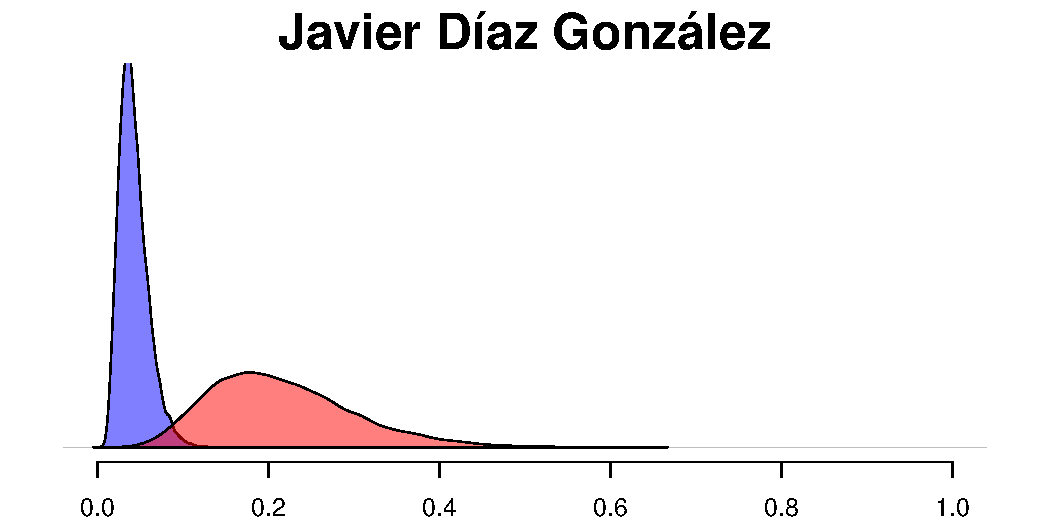
\includegraphics[width=.3\columnwidth]{../graphs/prReconoce1.pdf} &
    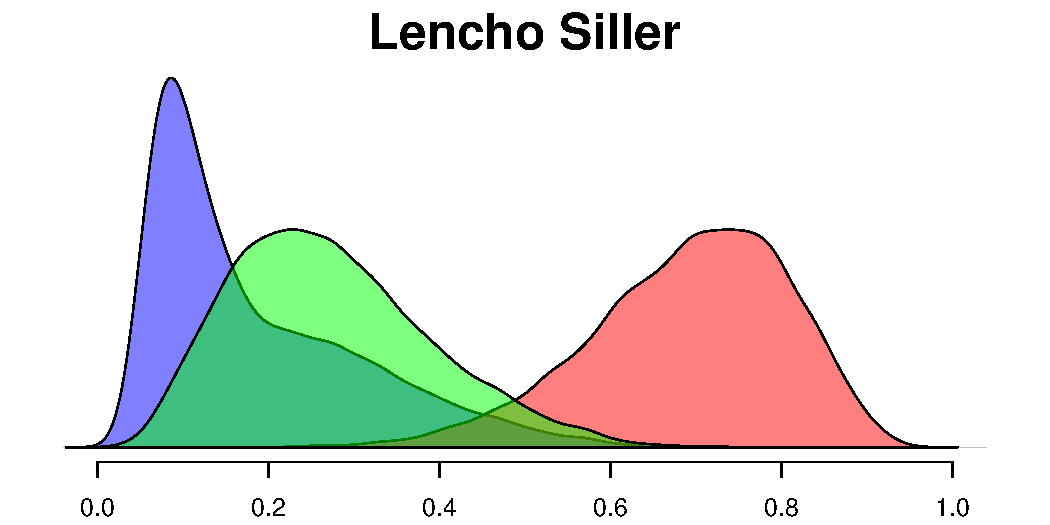
\includegraphics[width=.3\columnwidth]{../graphs/prReconoce6.pdf} &
    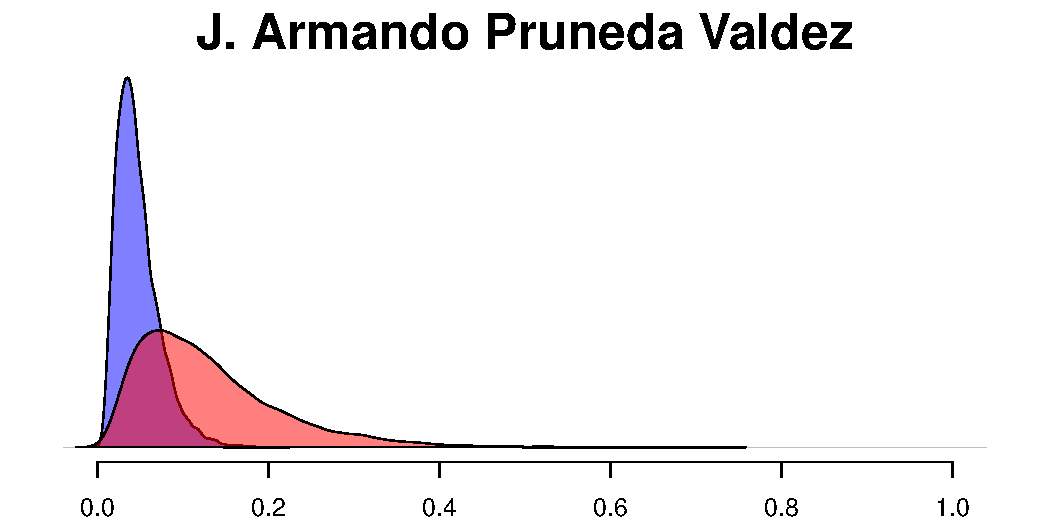
\includegraphics[width=.3\columnwidth]{../graphs/prReconoce8.pdf} \\
    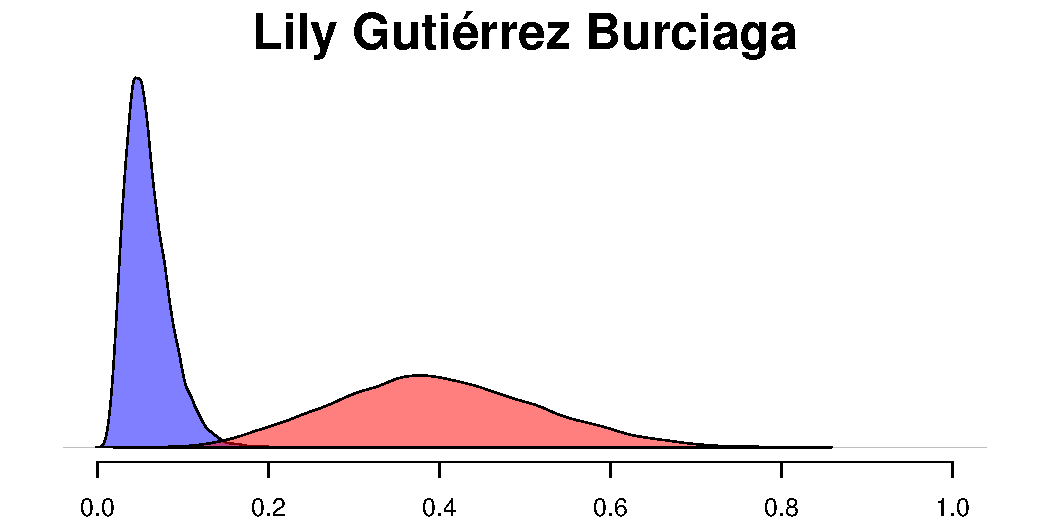
\includegraphics[width=.3\columnwidth]{../graphs/prReconoce2.pdf} &
    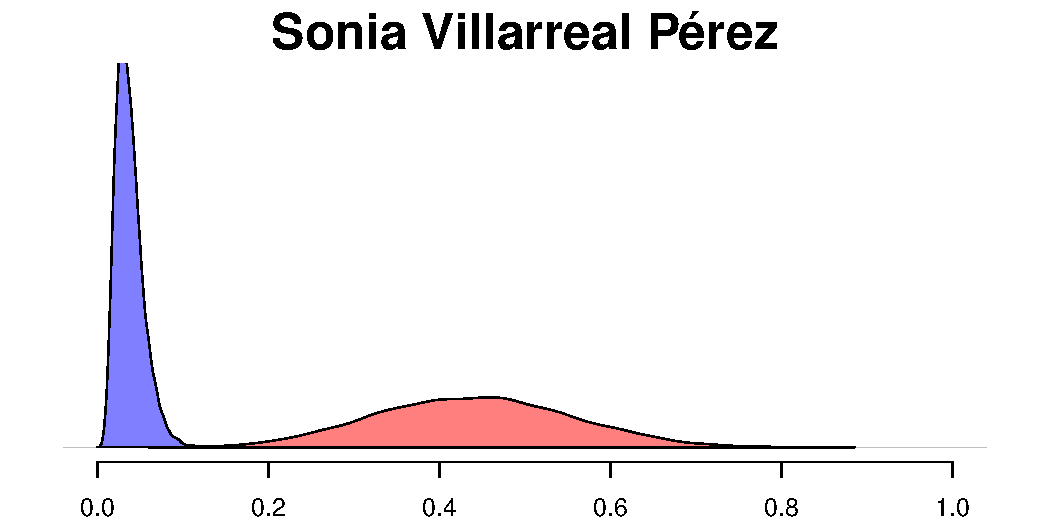
\includegraphics[width=.3\columnwidth]{../graphs/prReconoce5.pdf} &
    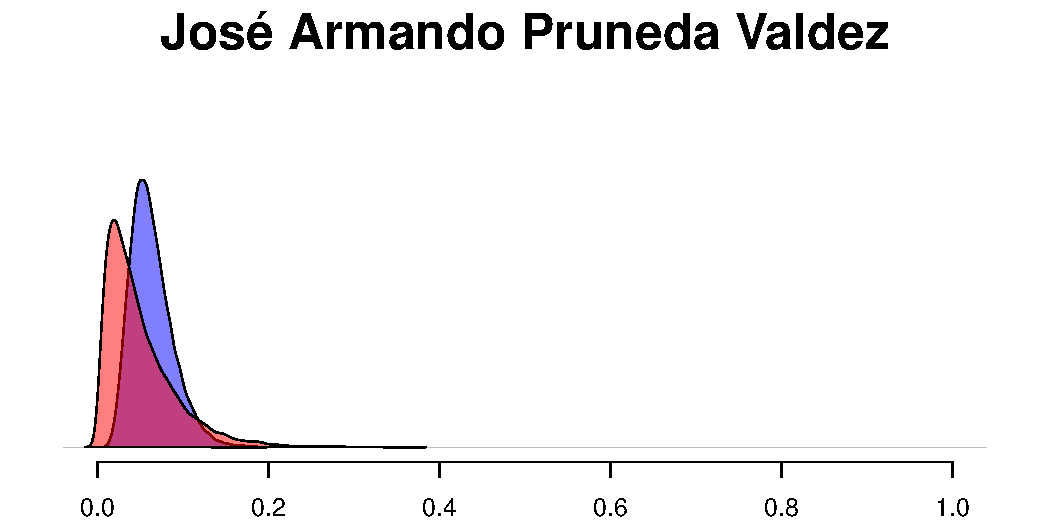
\includegraphics[width=.3\columnwidth]{../graphs/prReconoce7.pdf} \\
    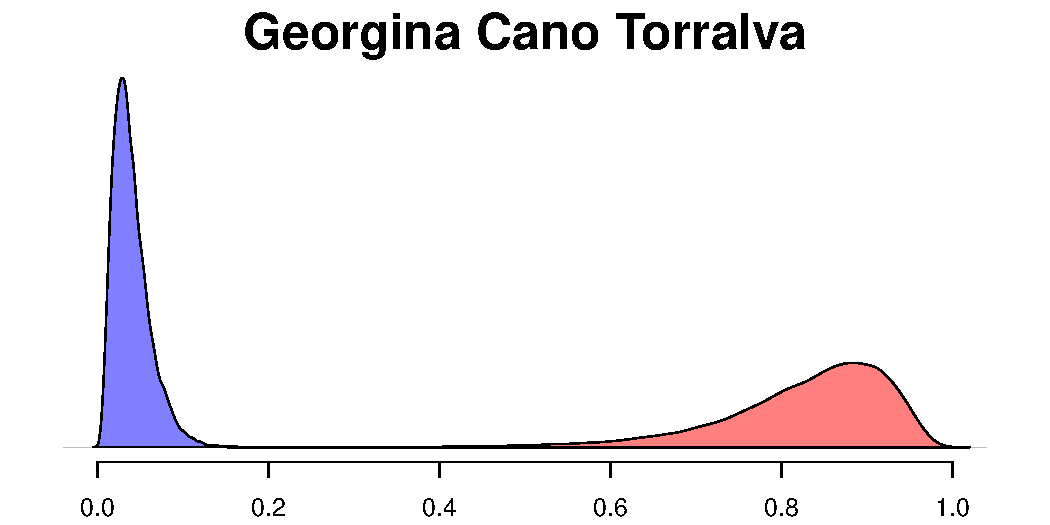
\includegraphics[width=.3\columnwidth]{../graphs/prReconoce3.pdf} &
    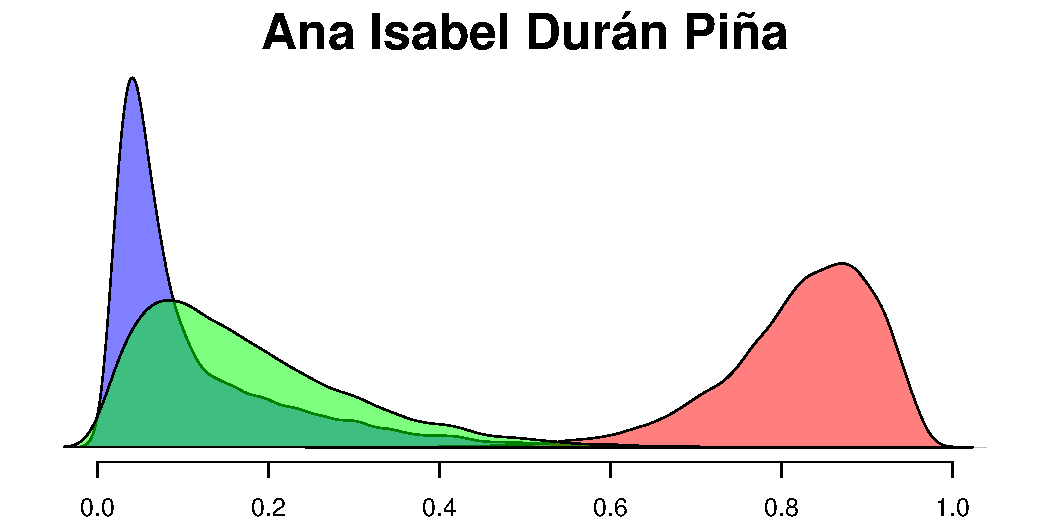
\includegraphics[width=.3\columnwidth]{../graphs/prReconoce4.pdf} &
    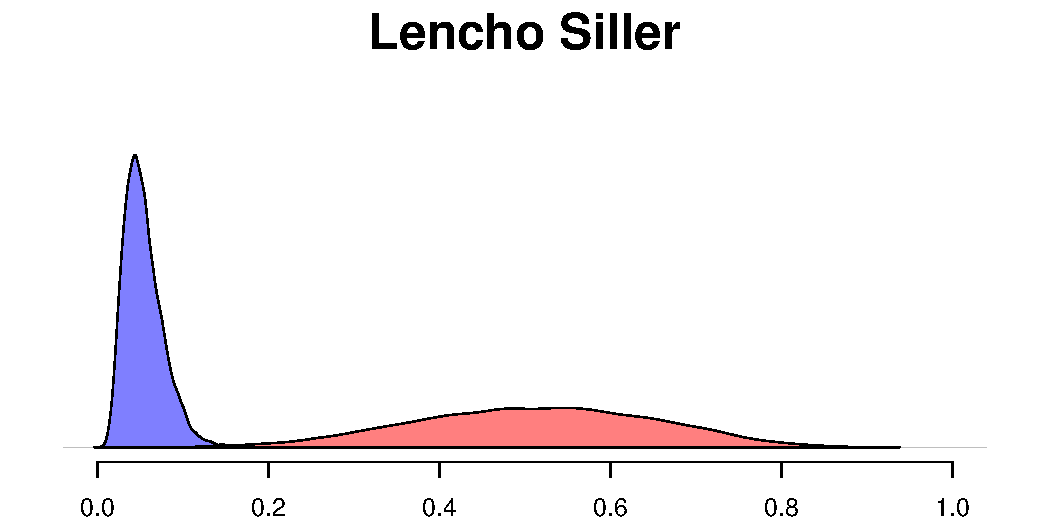
\includegraphics[width=.3\columnwidth]{../graphs/prReconoce9.pdf} \\
  \end{tabular}
  \caption{The probability of name recognition (x-axis). We portray simulations with Bayesian versions of regression models. The violet density is for respondents in area $n$, the green (when applicable) for respondents in area $l$, and the pink for respondents in area $r$. \emph{With clear gaps between them, we expect the purple to lie to the left, the pink to the right, the green between them}. All other controls held constant to represent a PAN-identifier with a smartphone, who said the incumbent has delivered but is uninterested in politics.}\label{f:sims}
\end{sidewaysfigure}

\section{Conclusion}

Despite an incomplete research design, we uncover evidence of name recognition consistent with the electoral connection model in Coahuila. 


\bibliographystyle{apsrInitials}
\bibliography{/home/eric/Dropbox/mydocs/magar}

\section*{Appendix}
\subsection{Regression results}

% Table created by stargazer v.5.2 by Marek Hlavac, Harvard University. E-mail: hlavac at fas.harvard.edu
% Date and time: Wed, Feb 14, 2018 - 08:56:20 PM
% Requires LaTeX packages: dcolumn 
\begin{sidewaystable}[!htbp] \centering 
%%\begin{tabular}{l|rrr|rrr|rrr} 
    \scalebox{.85}{
\begin{tabular}{@{\extracolsep{5pt}}lD{.}{.}{-3} D{.}{.}{-3} D{.}{.}{-3} D{.}{.}{-3} D{.}{.}{-3} D{.}{.}{-3} D{.}{.}{-3} D{.}{.}{-3} D{.}{.}{-3} } 
%\\[-1.8ex]\hline 
%\hline \\[-1.8ex] 
\\[-1.8ex] & \multicolumn{1}{c}{(1)} & \multicolumn{1}{c}{(2)} & \multicolumn{1}{c}{(3)} & \multicolumn{1}{c}{(4)} & \multicolumn{1}{c}{(5)} & \multicolumn{1}{c}{(6)} & \multicolumn{1}{c}{(7)} & \multicolumn{1}{c}{(8)} & \multicolumn{1}{c}{(9)}\\ 
  & \multicolumn{1}{c}{Javier} & \multicolumn{1}{c}{Lily} & \multicolumn{1}{c}{Gina} & \multicolumn{1}{c}{Lencho} & \multicolumn{1}{c}{Sonia} & \multicolumn{1}{c}{A.Isabel} & \multicolumn{1}{c}{Armando} & \multicolumn{1}{c}{Lariza} & \multicolumn{1}{c}{Leonel}\\ 
\hline \\[-1.8ex] 
 $\texttt{retained}$   & 1.85^{***} & 2.37^{***} & 4.91^{***} & 3.10^{***} & 3.02^{***} & 4.59^{***} & 1.10^{*} & -.22 & 2.93^{***} \\ 
  & (.33) & (.33) & (.41) & (.43) & (.32) & (.44) & (.58) & (.75) & (.38) \\ 
  & & & & & & & & & \\ 
 $\texttt{lost}$       & 1.29^{*} &  &  & 1.27^{***} &  & 1.46^{*} &  &  &  \\ 
  & (.68) &  &  & (.47) &  & (.81) &  &  &  \\ 
  & & & & & & & & & \\ 
 $\texttt{delivered}$  & .86^{***} & .76^{***} & 1.46^{***} & .51^{*} & .93^{***} & .26 & .51 & .85^{***} & .26 \\ 
  & (.25) & (.27) & (.34) & (.30) & (.27) & (.34) & (.37) & (.27) & (.33) \\ 
  & & & & & & & & & \\ 
 $\texttt{interested}$ & .35 & 1.03^{***} & 1.34^{***} & .82^{***} & .52^{**} & .74^{**} & .71^{**} & .28 & .57^{*} \\ 
  & (.24) & (.27) & (.34) & (.28) & (.26) & (.33) & (.36) & (.27) & (.31) \\ 
  & & & & & & & & & \\ 
 $\texttt{smartphone}$ & -.27 & .37 & -.18 & -.47^{*} & .21 & -.05 & -.43 & .26 & -.42 \\ 
  & (.24) & (.27) & (.31) & (.28) & (.26) & (.31) & (.35) & (.27) & (.30) \\ 
  & & & & & & & & & \\ 
 $\texttt{panista}$    & .15 & -.11 & -.03 & 1.18^{***} & .02 & .80^{*} & .78^{*} & .34 & 1.15^{***} \\ 
  & (.39) & (.41) & (.52) & (.35) & (.41) & (.44) & (.47) & (.39) & (.41) \\ 
  & & & & & & & & & \\ 
 $\texttt{priista}$    & .37 & .15 & -.01 & -.21 & .17 & .74^{**} & .43 & .19 & .16 \\ 
  & (.28) & (.30) & (.38) & (.37) & (.29) & (.35) & (.41) & (.31) & (.39) \\ 
  & & & & & & & & & \\ 
 $\texttt{morenista}$  & -.07 & .59 & .26 & .76 & -1.17 &  & -.26 & -1.01 & .88 \\ 
  & (.63) & (.51) & (.74) & (.55) & (1.04) &  & (1.05) & (1.03) & (.56) \\ 
  & & & & & & & & & \\ 
 Intercept             & -3.03^{***} & -3.82^{***} & -4.45^{***} & -3.48^{***} & -3.49^{***} & -3.99^{***} & -3.87^{***} & -3.29^{***} & -3.58^{***} \\ 
  & (.25) & (.30) & (.39) & (.30) & (.28) & (.35) & (.37) & (.28) & (.30) \\ 
  & & & & & & & & & \\ 
\hline \\[-1.8ex] 
Observations & \multicolumn{1}{c}{1,008} & \multicolumn{1}{c}{1,008} & \multicolumn{1}{c}{1,008} & \multicolumn{1}{c}{1,008} & \multicolumn{1}{c}{1,008} & \multicolumn{1}{c}{1,008} & \multicolumn{1}{c}{1,008} & \multicolumn{1}{c}{1,008} & \multicolumn{1}{c}{1,008} \\ 
Log Likelihood & \multicolumn{1}{c}{-262.32} & \multicolumn{1}{c}{-231.34} & \multicolumn{1}{c}{-169.84} & \multicolumn{1}{c}{-205.60} & \multicolumn{1}{c}{-235.20} & \multicolumn{1}{c}{-175.64} & \multicolumn{1}{c}{-147.10} & \multicolumn{1}{c}{-229.85} & \multicolumn{1}{c}{-182.89} \\ 
\hline 
\hline \\[-1.8ex] 
    \multicolumn{10}{r}{\footnotesize{$^{*}$p$<$.1; $^{**}$p$<$.05; $^{***}$p$<$.01}} \\ %[-1.8ex]
\end{tabular}
}
  \caption{Regression results. All models estimated with logit, standard errors in parentheses.} 
  \label{T:regs} 
\end{sidewaystable} 

\subsection{Survey questions}
Thirteen items in the survey questionnaire involved reelection and name recognition (from question 20 to question 25.i) . We used questions 25.a--25.i to code our dependent variables. Responses much/some/little (\emph{mucho/algo/poco}) coded as 1 in the incumbent's name recognition indicator; 0 otherwise.

* Add descriptives. 

We reproduce the relevant items in Spanish here.

\begin{footnotesize}
\begin{verbatim}
20 ¿Está usted a favor, en contra o le es indiferente la reelección 
consecutiva de legisladores?

1) A favor 2) En contra
3) Le es indiferente
4) NS/NC

21 El 3 de abril iniciaron las campañas para renovar el Congreso del Estado. 
Si yo le preguntara los nombres de los candidatos a diputado en este 
distrito, ¿usted me podría decir todos los nombres, algunos nombres o no 
recuerda ningún nombre en este momento?

1) Todos 2) Algunos
3) No recuerda
4) No contestó

22 Ahora piense por favor en los diputados locales actuales. Si yo le 
preguntara las cosas que ha hecho su diputado por esta comunidad, ¿usted 
podría mencionarme muchas cosas, algunas, diría que no hizo nada o no 
recuerda en este momento? [5=NS/NC]

1) Muchas
2) Algunas
3) No hizo nada
4) No recuerda

23 Si su actual diputado compitiera para buscar la reelección,
¿usted votaría por él o no votaría por él?

1) Sí votaría por él
2) No votaría por él
3) NS/NC (NO LEER)

24 Con base en el trabajo realizado por su actual diputado,
¿cree que merecería ser reelecto en su cargo o no?

[1=Sí; 2=No; 3=NC]

25 Le voy a leer unos nombres, para cada uno, ¿podría decirme si le es muy 
conocido, algo conocido, poco o nada conocido?

[1=Muy conocido; 2=Algo; 3=Poco; 4=Nada conocido; 5=NS/NC]

a Javier Díaz González     
b Lily Gutiérrez Burciaga  
c Georgina Cano Torralva   
d Ana Isabel Durán         
e Sonia Villareal          
f Lariza Montiel           
g Armando Pruneda          
h Leonel Contreras Pámanes 
i Florencio ``Lencho'' Siller
\end{verbatim}
\end{footnotesize}

\end{document}
